\section{Архитектура разработанной модели}

\subsection{Система сбора, анализа и мониторинга данных с устройств}

(Системный подход (Анатолий Левенчук))

(Микросервисная архитектура)

(Архитектура системы с кодовым названием Система 2.0)

\begin{figure}[h]
    \center{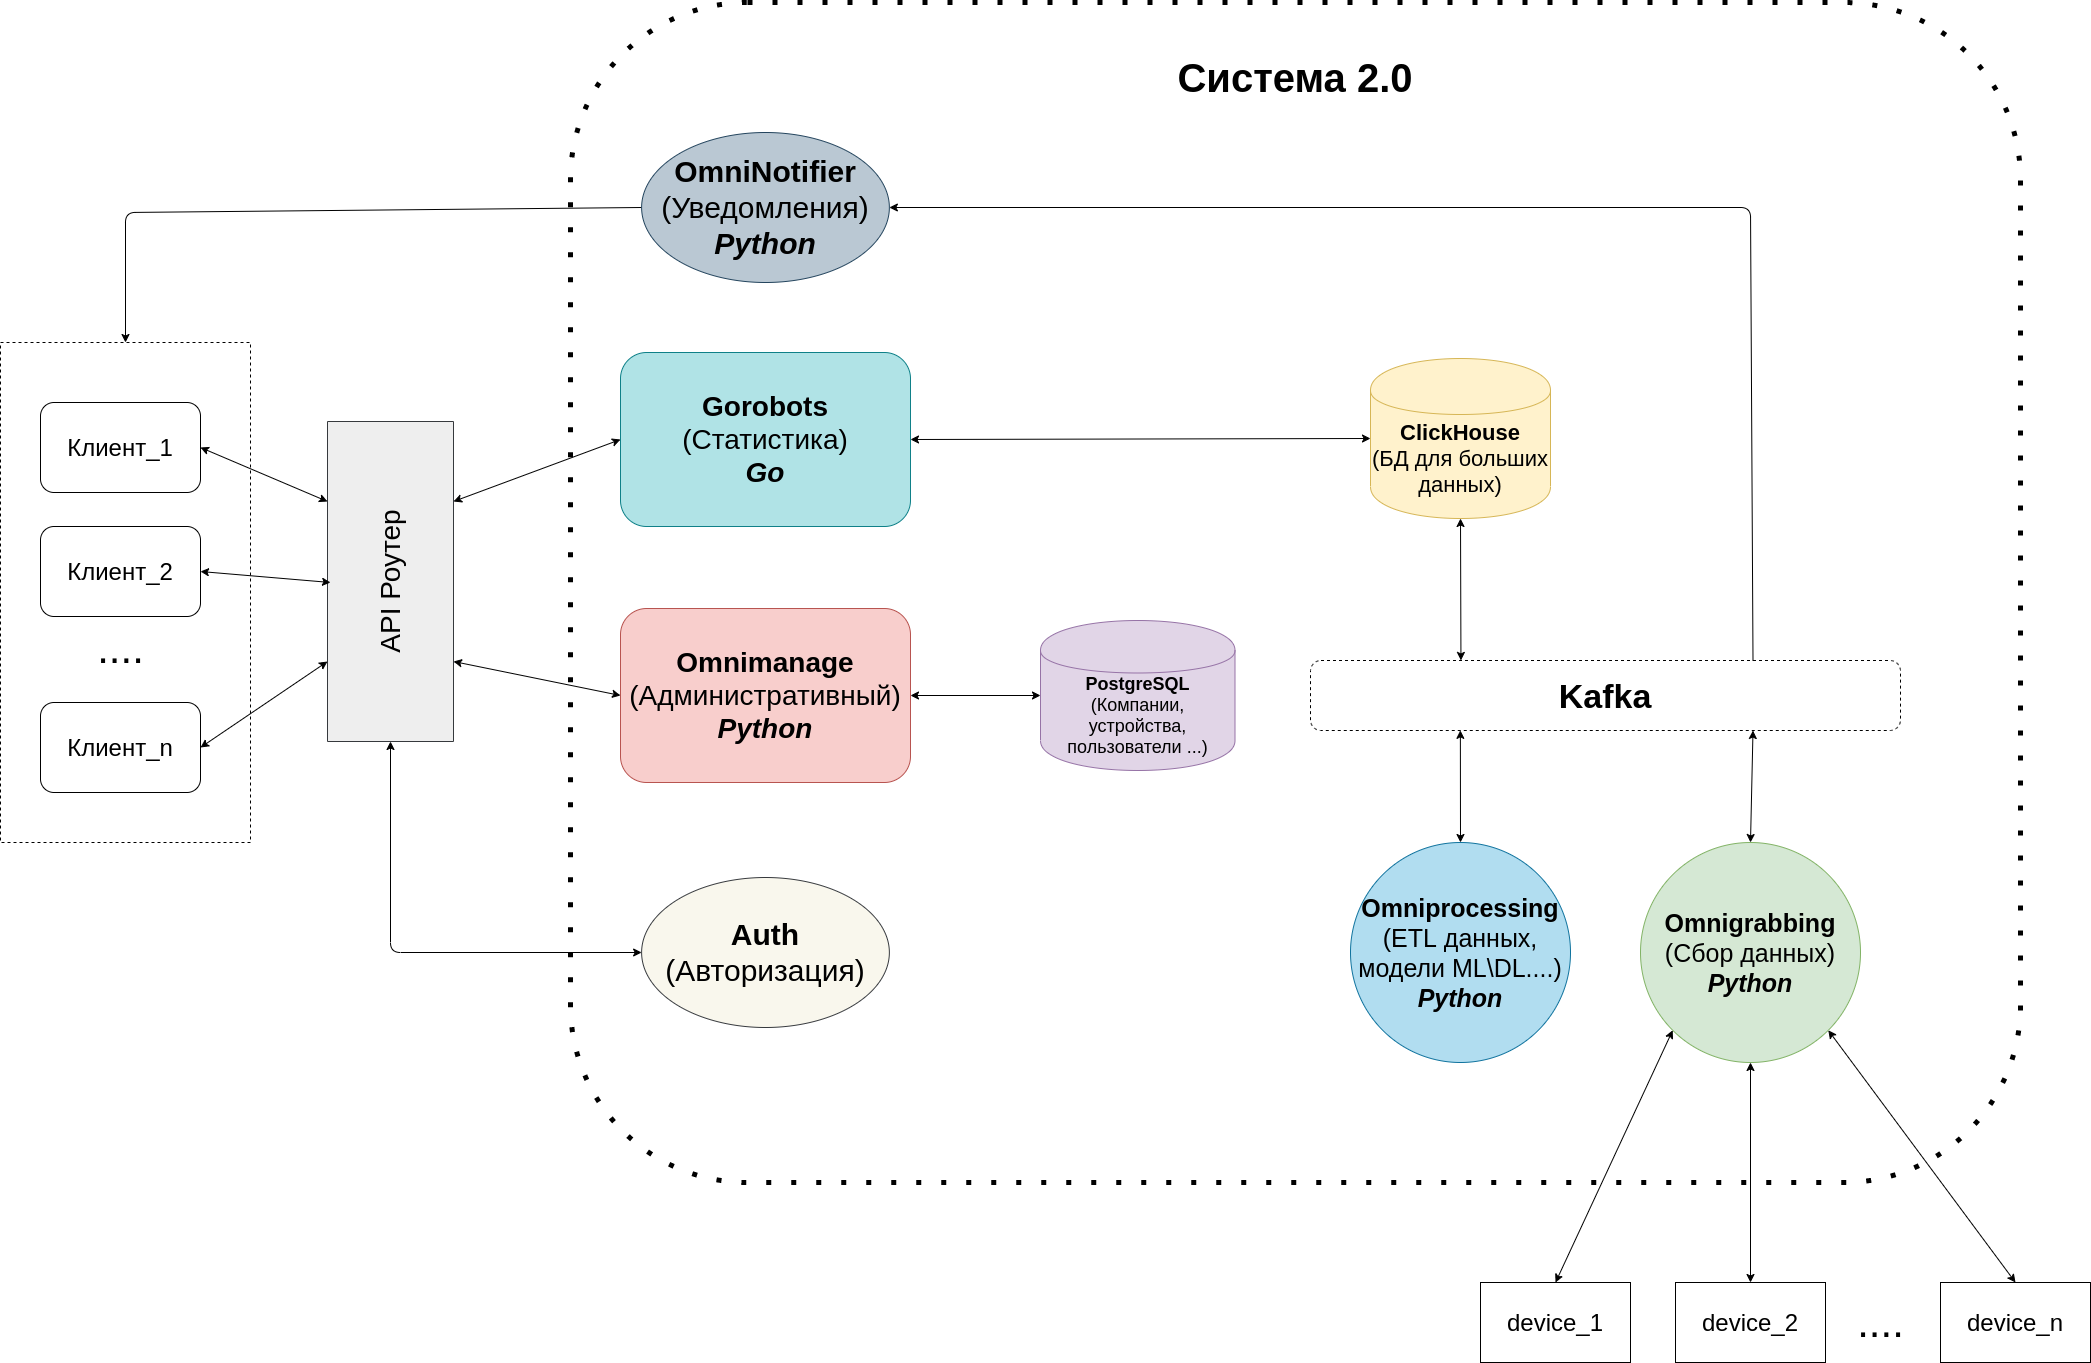
\includegraphics[width=15cm]{img/sys2.png}}
    \caption{Разработанная система для промышленного интернета вещей}
\end{figure}

(Описание микросервисов)

(Развертывание через Docker и Kubernetes)

\subsection{Место модели в системе}

Микросервис omniprocessing является местом, где расположена реализованная модель.
Основные цели данного микросервиса -- извлечение, трансформация и загрузка.

В omniprocessing используется Python фреймфорк Faust, который позволяет отправлять
данные в очередь брокеру сообщений Kafka. Из Kafka данные попадают в базу данных ClickHouse.
Благодаря данному фреймворку можно быстро строить и встраивать пайплайны машинного обучения. (ссылка)

(Kafka: описание и обонование использования)

(ClickHouse: описание и обоснование выбора)

(Faust: описание фреймворка и обоснование выбора)

(Место модели в микросервисе)


\subsection{Структура модели}

(Функциональное и модульное описание модели)

\clearpage